\documentclass[11pt, a4paper]{article}\usepackage[]{graphicx}\usepackage[]{color}
%% maxwidth is the original width if it is less than linewidth
%% otherwise use linewidth (to make sure the graphics do not exceed the margin)
\makeatletter
\def\maxwidth{ %
  \ifdim\Gin@nat@width>\linewidth
    \linewidth
  \else
    \Gin@nat@width
  \fi
}
\makeatother

\definecolor{fgcolor}{rgb}{0.345, 0.345, 0.345}
\newcommand{\hlnum}[1]{\textcolor[rgb]{0.686,0.059,0.569}{#1}}%
\newcommand{\hlstr}[1]{\textcolor[rgb]{0.192,0.494,0.8}{#1}}%
\newcommand{\hlcom}[1]{\textcolor[rgb]{0.678,0.584,0.686}{\textit{#1}}}%
\newcommand{\hlopt}[1]{\textcolor[rgb]{0,0,0}{#1}}%
\newcommand{\hlstd}[1]{\textcolor[rgb]{0.345,0.345,0.345}{#1}}%
\newcommand{\hlkwa}[1]{\textcolor[rgb]{0.161,0.373,0.58}{\textbf{#1}}}%
\newcommand{\hlkwb}[1]{\textcolor[rgb]{0.69,0.353,0.396}{#1}}%
\newcommand{\hlkwc}[1]{\textcolor[rgb]{0.333,0.667,0.333}{#1}}%
\newcommand{\hlkwd}[1]{\textcolor[rgb]{0.737,0.353,0.396}{\textbf{#1}}}%

\usepackage{framed}
\makeatletter
\newenvironment{kframe}{%
 \def\at@end@of@kframe{}%
 \ifinner\ifhmode%
  \def\at@end@of@kframe{\end{minipage}}%
  \begin{minipage}{\columnwidth}%
 \fi\fi%
 \def\FrameCommand##1{\hskip\@totalleftmargin \hskip-\fboxsep
 \colorbox{shadecolor}{##1}\hskip-\fboxsep
     % There is no \\@totalrightmargin, so:
     \hskip-\linewidth \hskip-\@totalleftmargin \hskip\columnwidth}%
 \MakeFramed {\advance\hsize-\width
   \@totalleftmargin\z@ \linewidth\hsize
   \@setminipage}}%
 {\par\unskip\endMakeFramed%
 \at@end@of@kframe}
\makeatother

\definecolor{shadecolor}{rgb}{.97, .97, .97}
\definecolor{messagecolor}{rgb}{0, 0, 0}
\definecolor{warningcolor}{rgb}{1, 0, 1}
\definecolor{errorcolor}{rgb}{1, 0, 0}
\newenvironment{knitrout}{}{} % an empty environment to be redefined in TeX

\usepackage{alltt}  
\usepackage[T1]{fontenc}               	% Vise norske tegn.
\usepackage[utf8]{inputenc}						% For ?f¥ kunne skrive norske tegn.
%\usepackage[norsk]{babel}								% Tilpasning til norsk.
\usepackage{graphicx}       						% For ?f¥ inkludere figurer.
\usepackage{subcaption}
\usepackage{amsmath,amssymb} 						% Ekstra matematikkfunksjoner.
\usepackage{indentfirst}                % For å få oppgaevbokstavene til å se pene ut
\usepackage{siunitx}							      % M?f¥ inkluderes for blant annet ?f¥ f?f¥ tilgang til kommandoen \SI (korrekte m?f¥ltall med enheter)
%\usepackage{textcomp}
%	\sisetup{exponent-product = \cdot}      % Prikk som multiplikasjonstegn (i steden for kryss).
% 	\sisetup{output-decimal-marker  =  {,}} % Komma som desimalskilletegn (i steden for punk
% 	\sisetup{separate-uncertainty = true}   % Pluss-minus-form p?f¥ usikkerhet (i steden for p
\usepackage{booktabs}                     % For ?f¥ f?f¥ tilgang til finere linjer (til bruk i tabeller og sli
\usepackage[font=small,labelfont=bf]{caption}	% For justering av figurtekst og tabelltekst.


% Disse kommandoene kan gj?f¸re det enklere for LaTeX ?f¥ plassere figurer og tabeller der du ?
\setcounter{totalnumber}{5}
\renewcommand{\textfraction}{0.05}
\renewcommand{\topfraction}{0.95}
\renewcommand{\bottomfraction}{0.95}
\renewcommand{\floatpagefraction}{0.35}
\newcommand{\tab}{\hspace*{2em}}
\renewcommand{\labelitemi}{$ $}



\author{Navn Navnesen}

\title{{\bf TMA4195} Mathematical Modelling Project}
\IfFileExists{upquote.sty}{\usepackage{upquote}}{}
\begin{document}

\maketitle

\section*{Deriving the modelling equations}
\subsection*{Diffusion equation}
Flux $J$:
\begin{align*}
J = -D\nabla c
\end{align*}


\begin{align*}
c_t = \kappa \Delta c\\
\frac{dc}{dt} = \kappa \nabla^2 c
\end{align*}
Neumann BC:
\begin{align*}
\nabla c \cdot n = g(t,c)
\end{align*}

\subsection*{The binding process}

First we look at the reversible chemical reaction

\begin{align*}
\text{R} + \text{N} \rightleftharpoons \text{RN}
\end{align*}

with reaction rate $k_1^*$ to the right and $k_2^*$ to the left, being respectively the probability for the reactions to occur in their direction. 
We get 3 ODE's from this chemical reaction:

\begin{align*}
\frac{d[\text{R}]}{dt} &= -k_1^*[\text{R}][\text{N}] + k_2^*[\text{RN}],\\
\frac{d[\text{N}]}{dt} &= -k_1^*[\text{R}][\text{N}] + k_2^*[\text{RN}],\\
\frac{d[\text{RN}]}{dt} &= k_1^*[\text{R}][\text{N}] - k_2^*[\text{RN}],
\end{align*}
where [R], [N] and [RN] are the concentratinos of the receptors, neurotransmitters and the bound product of them.
We may consider [N][R] the probability of a neurotransmitter meeting an unoccupied receptor, and $\bar{k}_1^*$ the probability of the binding reaction happening. Likewise for $\bar{k}_2^*$. $P^R$ is the probability of a receptor being unoccupied, $(1-P^R)$ the probability that the neurotransmitter is attatched to the receptor, leeds to the following simplification of the above ODE's:

\begin{align*}
\frac{d[\text{N}]}{dt} &= -\bar{k}_1^*[\text{N}]P^R + \bar{k}_2^*(1-P^R),\\
\frac{dP^R}{dt} &= -\bar{k}_1^*[\text{N}]P^R + \bar{k}_2^*(1-P^R).\\
\end{align*}

If we assume that the receptors are not uniformly distributed, we need to introduce a $\gamma(x)$ to describe the density of receptors.
At the boundary:
\begin{align*}
\frac{d[\text{N}]}{dt} &= -\bar{k}_1^*[\text{N}]\gamma P^R + \bar{k}_2^*\gamma(1-P^R),\\
\frac{dP^R}{dt} &= -\bar{k}_1^*[\text{N}]\gamma P^R + \bar{k}_2^*\gamma(1-P^R),\\
\end{align*}
which are Neumann boundary conditions (inserting $c$ for [N])

\begin{align*}
\kappa \nabla c \cdot n &= -\bar{k}_1^*c\gamma P^R + \bar{k}_2^*\gamma(1-P^R),\\
\frac{dP^R}{dt} &= -\bar{k}_1^*c P^R + \bar{k}_2^*(1-P^R),\\
\end{align*}

\subsection*{Glia cells}


\begin{align*}
\text{T} + \text{N} \rightleftharpoons \text{TN} \rightarrow \text{N}_{\text{inactive}} + \text{T}
\end{align*}
Define $k_3, k_4, k_5$ as the reaction rates of first rightward, first leftward, second rightward equation.

Similarly to the binding process, we get the following sets of equations:

\begin{align*}
\kappa \nabla c \cdot n &= -\bar{k}_3c\gamma^T P^T + \bar{k}_4\gamma^T(1-P^T),\\
\frac{dP^T}{dt} &= -\bar{k}_3c P^T + (1-P^T)(\bar{k}_4 + \bar{k}_5),\\
\end{align*}


Combining these equations, we get

\begin{align*}
\kappa \nabla c \cdot n &= -c(\bar{k}_1^*\gamma^R P^R + \bar{k}_3\gamma^T P^T) + \bar{k}_2^*\gamma^R (1-P^R) + \bar{k}_4\gamma^T (1-P^T)    ,\\
\frac{dP^R}{dt} &= -c\bar{k}_1^* P^R + \bar{k}_2^*(1-P^R),\\
\frac{dP^T}{dt} &= -c\bar{k}_3 P^T + (\bar{k}_4 + \bar{k}_5)(1-P^T),\\
\end{align*}


\section*{1D solution using solver}
Modelling the equation in one dimension is done by considering the points $a$ and $b$, and the line between them.  In this case, $a$ is on one side of the synaptic cleft, and $b$ is on the other side.  Due to this, the boundary conditions for $a$ and $b$ differ.  For $a$, we have 
\begin{align*}
\kappa \nabla c &= -{k}_3cP^T + {k}_4(1-P^T),\\
\end{align*}
and for $b$ we have
\begin{align*}
\kappa \nabla c &= -{k}_1c P^R + {k}_2(1-P^R).\\
\end{align*}
The next step is to combine these boundary conditions with the modelling equation to form a matrix equation.

%\subsection*{Mass matrix}
%The mass matrix was found to be \\
%\\
%$
%M_{N,N} =
% \begin{bmatrix}
%  \frac{h}{3}       & \frac{h}{6}    & 0           & \cdots           & \cdots           & 0 \\
%  \frac{h}{6}       & \frac{2h}{3}   & \ddots      & \ddots           & \cdots           & \vdots \\
%  0                 & \ddots         & \ddots      & \ddots           & \ddots           & \vdots  \\
%  \vdots            & \ddots         & \ddots      & \ddots           & \ddots           & 0  \\
%  \vdots            & \vdots         & \ddots      & \ddots           & \frac{2h}{3}     & \frac{h}{6}  \\
%  0                 & \cdots         & \cdots      & 0                & \frac{h}{6}      & \frac{h}{3}
% \end{bmatrix},\\
%$
%while the stiffness matrix was\\
%$
%K_{N,N} =
% \begin{bmatrix}
%  \frac{1}{h}        & -\frac{1}{h}    & 0           & \cdots           & \cdots            & 0 \\
%  -\frac{1}{h}       & \frac{2}{h}     & \ddots      & \ddots           & \cdots            & \vdots \\
%  0                  & \ddots          & \ddots      & \ddots           & \ddots            & \vdots  \\
%  \vdots             & \ddots          & \ddots      & \ddots           & \ddots            & 0  \\
%  \vdots             & \vdots          & \ddots      & \ddots           & \frac{2}{h}       & -\frac{1}{h}  \\
%  0                  & \cdots          & \cdots      & 0                & -\frac{1}{h}      & \frac{1}{h}
% \end{bmatrix}.\\
%$
The final equation was 
\begin{align*}
\hat{M}\dot{X}(t) = -\kappa\hat{K}X(t) - k_3\hat{Q}^a(X(t))X(t)  + k_4(1-X_{N+1}(t))\hat{d}^a \\
+ (k_4 + k_5)(1-X_{N+1}(t))\hat{e}^a - k_1\hat{Q}^b(X(t))X(t) + k_2(1-X_{N-2}(t))\hat{d}^b,\\
\end{align*}
and was found by Jorg Henrik Holstad \footnote{Jorg Henrik Holstad. (2011). Modellering av Diffusjon av Nevrotransmittere i den Ekstracellelaere Vaesken. Retrieved from https://www.duo.uio.no/bitstream/handle/10852/10871/MasteroppgaveHenrikHolstad.pdf}
Here, X is a vector of length N + 2, consisting of the concentrations at the nodes, as well as the probabilities $P_a^T$ and $P_b^R$:
$
X =
 \begin{bmatrix}
  C        \\
  P_a^T    \\
  P_b^R    \\
 \end{bmatrix}.\\
$
A plot using N = 9 internal nodes is shown below:

\begin{figure}[h!]
  \centering
    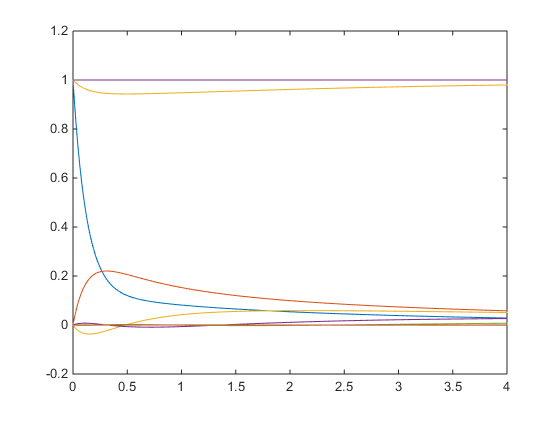
\includegraphics{ode45Trimmed}
      \caption{a = 0, b = 8, N = 9, $k_1=k_2=k_3=k_4=k_5 = 0.5, P_a^T(0) = P_b^R(0) = 1$}
\end{figure}



\end{document}
